\documentclass[aspectratio=169]{beamer}

% -- Theme & colours ----------------------------------------------------------
\usetheme{Madrid}
\usecolortheme{default}
\definecolor{darkblue}{RGB}{15,52,96}
\definecolor{accentblue}{RGB}{52,152,219}
\definecolor{accentyellow}{RGB}{241,196,15}
\definecolor{codegreen}{RGB}{39,174,96}
\definecolor{tcpcolor}{RGB}{31,97,141}
\definecolor{quiccolor}{RGB}{30,132,73}
\definecolor{codebg}{RGB}{40,44,52}

\setbeamercolor{palette primary}{bg=darkblue,fg=white}
\setbeamercolor{palette secondary}{bg=darkblue!80,fg=white}
\setbeamercolor{palette tertiary}{bg=darkblue!60,fg=white}
\setbeamercolor{palette quaternary}{bg=darkblue,fg=white}
\setbeamercolor{structure}{fg=accentblue}
\setbeamercolor{frametitle}{bg=darkblue,fg=white}
\setbeamercolor{block title}{bg=accentblue,fg=white}
\setbeamercolor{block body}{bg=accentblue!10}
\setbeamercolor{block title alerted}{bg=red!70!black,fg=white}
\setbeamercolor{block body alerted}{bg=red!10}
\setbeamercolor{block title example}{bg=codegreen!80!black,fg=white}
\setbeamercolor{block body example}{bg=codegreen!8}
\setbeamerfont{frametitle}{size=\large,series=\bfseries}
\setbeamertemplate{navigation symbols}{}

% -- Packages -----------------------------------------------------------------
\usepackage[utf8]{inputenc}
\usepackage[T1]{fontenc}
\usepackage{listings}
\usepackage{xcolor}
\usepackage{booktabs}
\usepackage{tikz}
\usepackage{array}
\usepackage{colortbl}
\usetikzlibrary{arrows.meta,positioning,fit,backgrounds}

% -- Listings style -----------------------------------------------------------
\lstdefinestyle{code}{
  backgroundcolor=\color{codebg},
  basicstyle=\ttfamily\scriptsize\color{white},
  keywordstyle=\color{accentblue}\bfseries,
  stringstyle=\color{accentyellow},
  commentstyle=\color{gray!60}\itshape,
  breaklines=true,
  frame=none,
  rulecolor=\color{gray},
  showstringspaces=false,
  tabsize=2,
  xleftmargin=0.5em,
  xrightmargin=0.5em,
  aboveskip=0.3em,
  belowskip=0.3em,
}
\lstset{style=code}

% -- Badge commands ------------------------------------------------------------
\newcommand{\tcpbadge}{\colorbox{tcpcolor}{\color{white}\tiny\textbf{~TCP~}}}
\newcommand{\quicbadge}{\colorbox{quiccolor}{\color{white}\tiny\textbf{~QUIC~}}}
\newcommand{\pybadge}{\colorbox{violet!70!black}{\color{white}\tiny\textbf{~Python~}}}
\newcommand{\javabadge}{\colorbox{orange!70!black}{\color{white}\tiny\textbf{~Java~}}}

% -- Title ---------------------------------------------------------------------
\title[TCP vs QUIC]{\textbf{TCP vs QUIC}\\A Practical Comparison through Chat Applications}
\subtitle{Computer Networks Lab}
\author{Undergraduate Computer Networks Course}
\date{}

% -----------------------------------------------------------------------------
\begin{document}
% -----------------------------------------------------------------------------

% -- Title slide ---------------------------------------------------------------
\begin{frame}
\titlepage
\vspace{-1em}
\begin{center}
  \tcpbadge\quad\quicbadge\quad\pybadge\quad\javabadge
\end{center}
\end{frame}

% -- Agenda --------------------------------------------------------------------
\begin{frame}{Agenda}
  \tableofcontents
\end{frame}

\section{TCP --- Transmission Control Protocol}
\section{QUIC --- Quick UDP Internet Connections}
\section{Protocol Comparison}
\section{TCP Implementation}
\section{QUIC Implementation}
\section{Code Comparison}
\section{Key Takeaways}

% ===================================================== SECTION 1 --- TCP
\begin{frame}{TCP --- Transmission Control Protocol}
  \begin{columns}[T]
    \column{0.5\textwidth}
      \begin{block}{Core guarantees (RFC 793 / 9293)}
        \begin{itemize}
          \item Ordered delivery
          \item Reliable --- retransmission on loss
          \item Flow control (sliding window)
          \item Congestion control (slow start, AIMD)
        \end{itemize}
      \end{block}
    \column{0.5\textwidth}
      \begin{alertblock}{Limitations}
        \begin{itemize}
          \item 1 RTT for 3-way handshake
          \item \textbf{Head-of-line blocking} --- one lost packet stalls all data
          \item Connection tied to IP:port (no migration)
          \item TLS is a separate layer (+1 RTT)
        \end{itemize}
      \end{alertblock}
  \end{columns}
\end{frame}

% -- TCP handshake -------------------------------------------------------------
\begin{frame}{TCP --- Three-Way Handshake}
  \begin{columns}[T]
    \column{0.5\textwidth}
      \begin{center}
      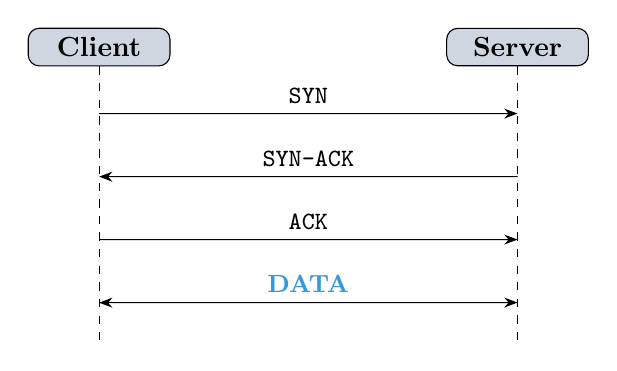
\begin{tikzpicture}[>=Stealth, node distance=1.4cm]
        \node (c) [draw, fill=darkblue!20, rounded corners, minimum width=1.8cm] {\textbf{Client}};
        \node (s) [draw, fill=darkblue!20, rounded corners, minimum width=1.8cm, right=3.5cm of c] {\textbf{Server}};

        \draw[->] ([yshift=-0.6cm]c.south) -- node[above,font=\small]{\texttt{SYN}} ([yshift=-0.6cm]s.south);
        \draw[<-] ([yshift=-1.4cm]c.south) -- node[above,font=\small]{\texttt{SYN-ACK}} ([yshift=-1.4cm]s.south);
        \draw[->] ([yshift=-2.2cm]c.south) -- node[above,font=\small]{\texttt{ACK}} ([yshift=-2.2cm]s.south);
        \draw[<->] ([yshift=-3.0cm]c.south) -- node[above,font=\small,color=accentblue]{\textbf{DATA}} ([yshift=-3.0cm]s.south);

        \draw[dashed] (c.south) -- ([yshift=-3.5cm]c.south);
        \draw[dashed] (s.south) -- ([yshift=-3.5cm]s.south);
      \end{tikzpicture}
      \end{center}
    \column{0.5\textwidth}
      \vspace{0.5em}
      \begin{block}{Connection overhead}
        \begin{itemize}
          \item 3 packets exchanged before any data
          \item \textbf{= 1 RTT overhead}
        \end{itemize}
      \end{block}
      \vspace{0.5em}
      \begin{block}{Adding TLS on top}
        \begin{tabular}{ll}
          TCP handshake & +1 RTT \\
          TLS 1.2       & +2 RTT \\
          TLS 1.3       & +1 RTT \\
          \hline
          \textbf{TLS 1.3 over TCP} & \textbf{2 RTT total} \\
        \end{tabular}
      \end{block}
      \vspace{0.5em}
      \begin{exampleblock}{}
        QUIC fixes this: transport + TLS in \textbf{1 RTT}
      \end{exampleblock}
\end{columns}
\end{frame}

% ===================================================== SECTION 2 --- QUIC
\begin{frame}{QUIC --- Quick UDP Internet Connections}
  \begin{columns}[T]
    \column{0.5\textwidth}
      \begin{block}{Design goals (RFC 9000, 2021)}
        \begin{itemize}
          \item Fix TCP's head-of-line blocking
          \item Faster connection setup (0--1 RTT)
          \item Encrypt everything by default
          \item Survive IP address changes
        \end{itemize}
      \end{block}
      \vspace{0.5em}
      \begin{exampleblock}{Used by}
        HTTP/3, YouTube, Google Search,\\
        Cloudflare, Meta, Apple iCloud
      \end{exampleblock}
    \column{0.5\textwidth}
      \begin{block}{How it works}
        \begin{itemize}
          \item Runs \textbf{over UDP} --- custom reliability
          \item \textbf{TLS 1.3 built-in} and mandatory
          \item \textbf{Multiple independent streams} per connection
          \item \textbf{Connection ID} --- survives NAT rebinding
        \end{itemize}
      \end{block}
      \vspace{0.5em}
      \begin{alertblock}{Key difference from TCP}
        A lost packet only blocks \emph{its own stream},\\
        not all other streams on the connection.
      \end{alertblock}
  \end{columns}
\end{frame}

% -- QUIC handshake ------------------------------------------------------------
\begin{frame}{QUIC --- Connection Setup \& Stream Model}
  \begin{columns}[T]
    \column{0.5\textwidth}
      \begin{center}
      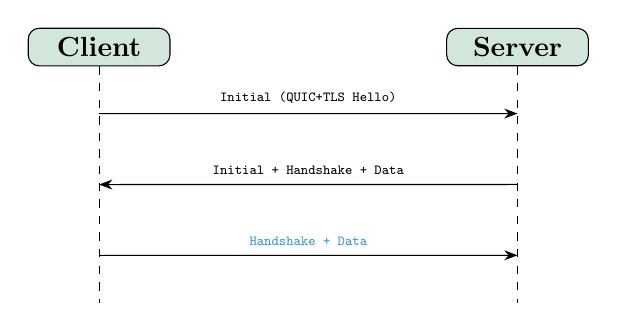
\begin{tikzpicture}[>=Stealth]
        \node (c) [draw, fill=quiccolor!20, rounded corners, minimum width=1.8cm] {\textbf{Client}};
        \node (s) [draw, fill=quiccolor!20, rounded corners, minimum width=1.8cm, right=3.5cm of c] {\textbf{Server}};

        \draw[->] ([yshift=-0.6cm]c.south) -- node[above,font=\tiny]{\texttt{Initial (QUIC+TLS Hello)}} ([yshift=-0.6cm]s.south);
        \draw[<-] ([yshift=-1.5cm]c.south) -- node[above,font=\tiny]{\texttt{Initial + Handshake + Data}} ([yshift=-1.5cm]s.south);
        \draw[->] ([yshift=-2.4cm]c.south) -- node[above,font=\tiny,color=accentblue]{\texttt{Handshake + \textbf{Data}}} ([yshift=-2.4cm]s.south);

        \draw[dashed] (c.south) -- ([yshift=-3cm]c.south);
        \draw[dashed] (s.south) -- ([yshift=-3cm]s.south);
      \end{tikzpicture}
      \end{center}
      \begin{exampleblock}{}
        \centering Transport + TLS in \textbf{1 RTT}
      \end{exampleblock}
    \column{0.5\textwidth}
      \textbf{QUIC stream types}\\[0.5em]
      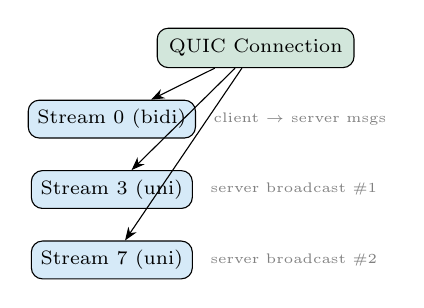
\begin{tikzpicture}[>=Stealth, font=\scriptsize]
        \node[draw, fill=quiccolor!20, rounded corners, minimum width=2.5cm, minimum height=0.5cm] (conn) {QUIC Connection};
        \node[draw, fill=accentblue!20, rounded corners, below left=0.4cm and -0.5cm of conn, minimum width=1.8cm] (s0) {Stream 0 (bidi)};
        \node[draw, fill=accentblue!20, rounded corners, below=0.4cm of s0, minimum width=1.8cm] (s1) {Stream 3 (uni)};
        \node[draw, fill=accentblue!20, rounded corners, below=0.4cm of s1, minimum width=1.8cm] (s2) {Stream 7 (uni)};
        \draw[->] (conn) -- (s0);
        \draw[->] (conn) -- (s1);
        \draw[->] (conn) -- (s2);
        \node[right=0.1cm of s0, font=\tiny, color=gray] {client $\to$ server msgs};
        \node[right=0.1cm of s1, font=\tiny, color=gray] {server broadcast \#1};
        \node[right=0.1cm of s2, font=\tiny, color=gray] {server broadcast \#2};
      \end{tikzpicture}
      \vspace{0.3em}
      \begin{itemize}
        \footnotesize
        \item Loss in stream 3 does \textbf{not} block stream 7
        \item Client-initiated or server-initiated
        \item Unidirectional or bidirectional
      \end{itemize}
  \end{columns}
\end{frame}

% ===================================================== SECTION 3 --- Comparison
\begin{frame}{TCP vs QUIC --- Protocol Comparison}
  \begin{center}
  \footnotesize
  \renewcommand{\arraystretch}{1.3}
  \begin{tabular}{>{\bfseries}l >{\tcpbadge~}l >{\quicbadge~}l}
    \toprule
    \textbf{Property} & \multicolumn{1}{c}{\tcpbadge\ TCP} & \multicolumn{1}{c}{\quicbadge\ QUIC} \\
    \midrule
    Runs over        & IP directly & UDP \\
    Connection setup & 1 RTT (3-way handshake) & 1 RTT (combined w/ TLS) \\
    Encryption       & Optional (TLS on top)  & Mandatory TLS 1.3 \\
    Streams/conn     & 1 ordered byte stream  & Many independent streams \\
    HoL blocking     & \textcolor{red!70!black}{Yes --- stalls all data} & \textcolor{codegreen}{No --- streams independent} \\
    Conn migration   & \textcolor{red!70!black}{No --- tied to IP:port} & \textcolor{codegreen}{Yes --- connection ID} \\
    Standard         & RFC 793 (1981) & RFC 9000 (2021) \\
    Used by          & HTTP/1.1, HTTP/2, SSH & HTTP/3, YouTube, CDNs \\
    \bottomrule
  \end{tabular}
  \end{center}
\end{frame}

% -- Chat app design -----------------------------------------------------------
\begin{frame}{Chat Application --- Architecture}
  \begin{columns}[T]
    \column{0.45\textwidth}
      \begin{center}
      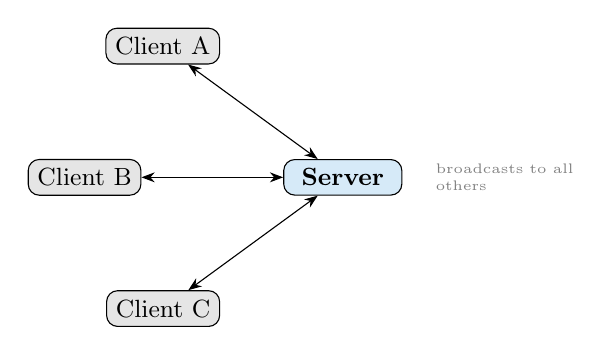
\begin{tikzpicture}[>=Stealth, font=\small]
        \node[draw, fill=accentblue!20, rounded corners, minimum width=1.5cm] (srv) {\textbf{Server}};
        \node[draw, fill=gray!20, rounded corners, above left=1.2cm and 0.8cm of srv] (a) {Client A};
        \node[draw, fill=gray!20, rounded corners, left=1.8cm of srv] (b) {Client B};
        \node[draw, fill=gray!20, rounded corners, below left=1.2cm and 0.8cm of srv] (c) {Client C};
        \draw[<->] (a) -- (srv);
        \draw[<->] (b) -- (srv);
        \draw[<->] (c) -- (srv);
        \node[right=0.3cm of srv, font=\tiny, text width=1.8cm, color=gray] {broadcasts to all others};
      \end{tikzpicture}
      \end{center}
    \column{0.55\textwidth}
      \begin{block}{Message flow}
        \begin{enumerate}\small
          \item Client connects and sends \textbf{name}
          \item Client sends a \textbf{message}
          \item Server \textbf{broadcasts} to all other clients
          \item Client disconnects --- server notifies others
        \end{enumerate}
      \end{block}
      \vspace{0.4em}
      \footnotesize
      \begin{tabular}{lll}
        \toprule
        \textbf{Protocol} & \textbf{Lang} & \textbf{Files} \\
        \midrule
        \tcpbadge & \pybadge & server\_tcp.py / client\_tcp.py \\
        \tcpbadge & \javabadge & ServerTCP.java / ClientTCP.java \\
        \quicbadge & \pybadge & server.py / client.py \\
        \quicbadge & \javabadge & ServerQUIC.java / ClientQUIC.java \\
        \bottomrule
      \end{tabular}
  \end{columns}
\end{frame}

% ===================================================== SECTION 4 --- TCP impl
\begin{frame}[fragile]{TCP Server --- Python \pybadge}
  \begin{columns}[T]
    \column{0.6\textwidth}
\begin{lstlisting}[language=Python]
# One coroutine handles one client connection
async def handle_client(reader, writer):
    conn_id = _alloc_id()
    _writers[conn_id] = writer

    while True:
        data = await reader.readline() # suspend until '\n'
        if not data:
            break                      # client disconnected

        text = data.decode().strip()
        if username is None:
            username = text            # first msg = display name
            _broadcast(f"*** {username} joined ***", conn_id)
        else:
            _broadcast(f"{username}: {text}", conn_id)

# start_server registers handle_client for every connection
server = await asyncio.start_server(handle_client, HOST, PORT)
\end{lstlisting}
    \column{0.4\textwidth}
      \begin{block}{Key points}
        \begin{itemize}\small
          \item \texttt{readline()} suspends --- other clients still run
          \item \texttt{b""} means connection closed
          \item First line = display name (app protocol)
          \item \textbf{No threads} --- coroutines share one thread
        \end{itemize}
      \end{block}
  \end{columns}
\end{frame}

\begin{frame}[fragile]{TCP Client --- Python \pybadge}
  \begin{columns}[T]
    \column{0.6\textwidth}
\begin{lstlisting}[language=Python]
# TCP 3-way handshake
reader, writer = await asyncio.open_connection(HOST, PORT)

# Task 1: receive broadcasts from server
async def receive_loop():
    while True:
        data = await reader.readline()
        print(data.decode().strip())

# Task 2: read keyboard and send to server
async def send_loop():
    while True:
        line = await loop.run_in_executor(None, stdin.readline)
        writer.write((line + "\n").encode())

# Run both concurrently; stop when either finishes
await asyncio.wait(
    [create_task(receive_loop()), create_task(send_loop())],
    return_when=FIRST_COMPLETED)
\end{lstlisting}
    \column{0.4\textwidth}
      \begin{block}{Key points}
        \begin{itemize}\small
          \item \texttt{open\_connection} does the handshake
          \item Two tasks run concurrently in \textbf{one thread}
          \item \texttt{run\_in\_executor} offloads blocking stdin to a thread pool
          \item Stop when user types \texttt{quit}
        \end{itemize}
      \end{block}
  \end{columns}
\end{frame}

\begin{frame}[fragile]{TCP Server --- Java \javabadge}
  \begin{columns}[T]
    \column{0.6\textwidth}
\begin{lstlisting}[language=Java]
// Accept loop --- one new thread per incoming connection
while (true) {
    Socket socket = serverSocket.accept(); // blocks
    int id = allocId();
    ClientHandler handler = new ClientHandler(socket, id);
    clients.put(id, handler);      // ConcurrentHashMap
    new Thread(handler).start();   // OS-scheduled thread
}

// Inside ClientHandler.run()
while ((line = reader.readLine()) != null) {
    if (username == null) {
        username = line;
        broadcast("*** " + username + " joined ***", connId);
    } else {
        broadcast(username + ": " + line, connId);
    }
}
\end{lstlisting}
    \column{0.4\textwidth}
      \begin{block}{Key points}
        \begin{itemize}\small
          \item \textbf{One thread per client} (preemptive)
          \item \texttt{ConcurrentHashMap} needed --- multiple threads access client list
          \item Python uses a plain dict --- safe because only 1 async thread
        \end{itemize}
      \end{block}
      \begin{exampleblock}{Python vs Java}
        \small Same protocol logic.\\
        Different concurrency model:\\ coroutines vs threads.
      \end{exampleblock}
  \end{columns}
\end{frame}

% ===================================================== SECTION 5 --- QUIC impl
\begin{frame}[fragile]{QUIC Server --- Python \pybadge}
  \begin{columns}[T]
    \column{0.6\textwidth}
\begin{lstlisting}[language=Python]
class ChatServerProtocol(QuicConnectionProtocol):

    # Called for every QUIC event on this connection
    def quic_event_received(self, event):
        if isinstance(event, StreamDataReceived):
            self._buf += event.data
            while b"\n" in self._buf:       # buffer until '\n'
                line, self._buf = self._buf.split(b"\n", 1)
                self._on_line(line.decode())

    # Broadcast: open a new stream per destination
    def _broadcast(self, message, exclude_id):
        for proto in active_connections.values():
            sid = proto._quic.get_next_available_stream_id(
                      is_unidirectional=True)
            proto._quic.send_stream_data(sid, data, end_stream=True)
            proto.transmit()          # flush UDP send buffer
\end{lstlisting}
    \column{0.4\textwidth}
      \begin{block}{vs TCP server}
        \begin{itemize}\small
          \item No \texttt{readline()} --- data arrives as \textbf{events}
          \item Must buffer bytes manually until \texttt{\textbackslash n}
          \item Each broadcast opens a \textbf{new QUIC stream}
          \item One class instance = one connection
        \end{itemize}
      \end{block}
      \begin{exampleblock}{}
        \small QUIC streams are cheap.\\Opening one per broadcast is normal and efficient.
      \end{exampleblock}
  \end{columns}
\end{frame}

\begin{frame}[fragile]{QUIC Client --- Python \pybadge}
  \begin{columns}[T]
    \column{0.6\textwidth}
\begin{lstlisting}[language=Python]
class ChatClientProtocol(QuicConnectionProtocol):
    # Server pushes messages via new streams --- handle here
    def quic_event_received(self, event):
        if isinstance(event, StreamDataReceived):
            text = event.data.decode().strip()
            print(f"\r{text}\n> ", end="", flush=True)
        else:
            super().quic_event_received(event)

# Configure: skip cert check (classroom demo)
config = QuicConfiguration(is_client=True)
config.verify_mode = ssl.CERT_NONE

async with connect(HOST, PORT, configuration=config,
                   create_protocol=ChatClientProtocol) as conn:
    reader, writer = await conn.create_stream() # bidi stream
    writer.write((username + "\n").encode())     # register name
\end{lstlisting}
    \column{0.4\textwidth}
      \begin{block}{Key points}
        \begin{itemize}\small
          \item Subclass \texttt{QuicConnectionProtocol}
          \item Server pushes via \texttt{StreamDataReceived}
          \item Outgoing: client opens a \textbf{bidirectional} stream
          \item \texttt{noServerCertificateCheck} skips TLS cert validation
        \end{itemize}
      \end{block}
  \end{columns}
\end{frame}

\begin{frame}[fragile]{QUIC Server --- Java \javabadge\ (kwik library)}
  \begin{columns}[T]
    \column{0.6\textwidth}
\begin{lstlisting}[language=Java]
// Factory: kwik calls createConnection() per new client
class ChatProtocolFactory
    implements ApplicationProtocolConnectionFactory {

  public ApplicationProtocolConnection createConnection(
        String protocol, QuicConnection conn) {
    return new ChatSession(idCounter.incrementAndGet(), conn);
  }
  public int maxConcurrentPeerInitiatedBidirectionalStreams() {
    return 10;
  }
}

// kwik calls this when client opens a stream
public void acceptPeerInitiatedStream(QuicStream stream) {
  new Thread(() -> {
    BufferedReader r = new BufferedReader(
        new InputStreamReader(stream.getInputStream()));
    while ((line = r.readLine()) != null)
        broadcast(username + ": " + line, connId);
  }).start();
}
\end{lstlisting}
    \column{0.4\textwidth}
      \begin{block}{Key points}
        \begin{itemize}\small
          \item \textbf{ALPN} \texttt{"chat"} is registered --- QUIC uses this during TLS handshake
          \item \texttt{acceptPeerInitiatedStream} $\approx$ \texttt{quic\_event\_received} in Python
          \item kwik wraps QUIC stream in \texttt{InputStream} --- feels like TCP!
          \item Broadcast: \texttt{createStream(false)} = unidirectional push
        \end{itemize}
      \end{block}
  \end{columns}
\end{frame}

% ===================================================== SECTION 6 --- Code compare
\begin{frame}[fragile]{Code Comparison --- Receiving Data}
  \begin{columns}[T]
    \column{0.5\textwidth}
      \textbf{\tcpbadge\ TCP --- Python}
\begin{lstlisting}[language=Python]
data = await reader.readline()
# blocks until '\n' arrives
text = data.decode().strip()
\end{lstlisting}

      \vspace{0.6em}
      \textbf{\tcpbadge\ TCP --- Java}
\begin{lstlisting}[language=Java]
String line = reader.readLine();
// blocks until '\n' arrives
\end{lstlisting}

    \column{0.5\textwidth}
      \textbf{\quicbadge\ QUIC --- Python}
\begin{lstlisting}[language=Python]
def quic_event_received(self, event):
    if isinstance(event, StreamDataReceived):
        self._buf += event.data
        while b"\n" in self._buf:
            line, self._buf = \
                self._buf.split(b"\n", 1)
\end{lstlisting}

      \vspace{0.4em}
      \textbf{\quicbadge\ QUIC --- Java (kwik)}
\begin{lstlisting}[language=Java]
// kwik wraps stream in InputStream
BufferedReader r = new BufferedReader(
  new InputStreamReader(
    stream.getInputStream()));
String line = r.readLine(); // like TCP!
\end{lstlisting}
  \end{columns}
  \begin{exampleblock}{}
    TCP gives a continuous byte stream. QUIC delivers data as \textbf{events} --- you must buffer. kwik's Java API hides this with \texttt{InputStream}.
  \end{exampleblock}
\end{frame}

\begin{frame}[fragile]{Code Comparison --- Broadcasting to Other Clients}
  \begin{columns}[T]
    \column{0.5\textwidth}
      \textbf{\tcpbadge\ TCP --- Python}
\begin{lstlisting}[language=Python]
for cid, writer in _writers.items():
    if cid == exclude: continue
    writer.write(data) # same TCP conn
\end{lstlisting}

      \vspace{0.5em}
      \textbf{\tcpbadge\ TCP --- Java}
\begin{lstlisting}[language=Java]
for (var e : clients.entrySet()) {
  if (e.getKey() == excludeId) continue;
  e.getValue().out.write(data); // same socket
  e.getValue().out.flush();
}
\end{lstlisting}

    \column{0.5\textwidth}
      \textbf{\quicbadge\ QUIC --- Python}
\begin{lstlisting}[language=Python]
for proto in active_connections.values():
    sid = proto._quic \
        .get_next_available_stream_id(
            is_unidirectional=True)
    proto._quic.send_stream_data(
        sid, data, end_stream=True)
    proto.transmit()
\end{lstlisting}

      \vspace{0.3em}
      \textbf{\quicbadge\ QUIC --- Java}
\begin{lstlisting}[language=Java]
QuicStream s = connection.createStream(false);
s.getOutputStream()
 .write((msg + "\n").getBytes());
s.getOutputStream().close(); // end-of-stream
\end{lstlisting}
  \end{columns}
  \begin{exampleblock}{}
    TCP reuses one byte stream. QUIC opens a \textbf{new stream per broadcast} --- no head-of-line blocking between messages.
  \end{exampleblock}
\end{frame}

% -- Full comparison table -----------------------------------------------------
\begin{frame}{Implementation Comparison --- All Four Versions}
  \centering\footnotesize
  \renewcommand{\arraystretch}{1.25}
  \begin{tabular}{>{\bfseries}l cccc}
    \toprule
    & \tcpbadge\ Python & \tcpbadge\ Java & \quicbadge\ Python & \quicbadge\ Java \\
    \midrule
    Library    & asyncio      & java.net    & aioquic        & kwik \\
    Concurrency & Coroutines  & Threads     & Coroutines     & Threads \\
    Server listen & start\_server & ServerSocket & serve()   & ServerConnector \\
    Per-conn object & coroutine & Runnable & Protocol subclass & AppProtoConnection \\
    Receive data & readline() & readLine() & quic\_event\_received & acceptPeerInitiatedStream \\
    Send data   & writer.write & out.write  & send\_stream\_data & createStream+write \\
    TLS         & None        & None        & Auto cert      & keytool cert \\
    Extra deps  & None        & None        & aioquic        & kwik (Maven) \\
    \bottomrule
  \end{tabular}
\end{frame}

% ===================================================== SECTION 7 --- Takeaways
\begin{frame}{Key Takeaways}
  \begin{enumerate}
    \item<1-> \textbf{Same application logic, different transport API.}\\
      Broadcast chat works identically over TCP and QUIC --- only the API changes.

    \vspace{0.4em}
    \item<2-> \textbf{QUIC $\neq$ ``faster TCP''.}\\
      The main benefit is \emph{stream multiplexing} (no HoL blocking) and \emph{0/1-RTT setup}, not raw throughput.

    \vspace{0.4em}
    \item<3-> \textbf{QUIC always uses TLS 1.3.}\\
      The certificate is part of the protocol --- you cannot disable encryption.

    \vspace{0.4em}
    \item<4-> \textbf{Event-driven vs stream-driven.}\\
      TCP gives a continuous byte stream. QUIC delivers data as events. Libraries like kwik bridge this with \texttt{InputStream}.

    \vspace{0.4em}
    \item<5-> \textbf{Coroutines (Python) vs Threads (Java).}\\
      Both handle many clients concurrently --- different scheduling models.

    \vspace{0.4em}
    \item<6-> \textbf{QUIC is the future.}\\
      HTTP/3 (RFC 9114) is built on QUIC. Used by ${\sim}25\%$ of all web traffic today.
  \end{enumerate}
\end{frame}

% -- Try it --------------------------------------------------------------------
\begin{frame}[fragile]{Try It Yourself}
  \begin{columns}[T]
    \column{0.5\textwidth}
      \textbf{\tcpbadge\ TCP --- Python}
\begin{lstlisting}[language=bash]
python server_tcp.py
python client_tcp.py
\end{lstlisting}
      \vspace{0.5em}
      \textbf{\tcpbadge\ TCP --- Java}
\begin{lstlisting}[language=bash]
javac ServerTCP.java ClientTCP.java
java ServerTCP
java ClientTCP
\end{lstlisting}
    \column{0.5\textwidth}
      \textbf{\quicbadge\ QUIC --- Python}
\begin{lstlisting}[language=bash]
pip install aioquic cryptography
python server.py
python client.py
\end{lstlisting}
      \vspace{0.5em}
      \textbf{\quicbadge\ QUIC --- Java}
\begin{lstlisting}[language=bash]
cd quic_java && mvn package -q
java -cp target/quic-chat-*-jar-with-\
dependencies.jar ServerQUIC
java -cp target/quic-chat-*-jar-with-\
dependencies.jar ClientQUIC
\end{lstlisting}
  \end{columns}
  \vspace{0.5em}
  \begin{center}
    \small\texttt{github.com/ensarg/computer\_networks\_lab}
  \end{center}
\end{frame}

\end{document}
